\documentclass[runningheads]{llncs}

\usepackage[T1]{fontenc}
\usepackage{graphicx}
\usepackage{booktabs}

\begin{document}
    \title{...}
    \titlerunning{...}

    \author{...}
    \authorrunning{...}

    \institute {....}
    
    \maketitle 
    
    \begin{abstract}
        Detecting sarcasm in text is a complex challenge that has significant implications for natural language processing. This paper investigates various machine learning and deep 
        learning approaches to sarcasm detection, focusing on models with Term Frequency-Inverse Document Frequency (TF-IDF) and Bag-of-Words (BoW) representations, as well as 
        Long Short-Term Memory (LSTM) networks utilizing GloVe and Word2Vec embeddings. My results demonstrate that TF-IDF-based models achieve a favorable balance between accuracy and 
        misclassification rates, while LSTM models exhibit promising performance, with Word2Vec outperforming GloVe embeddings. The results highlight the importance of model selection and 
        feature representation in sarcasm detection models. I wish for this to provide baseline benchmarks for future research aimed at improving the computational understanding of sarcastic expressions.
    \end{abstract}
    
    \keywords{Sarcasm, Feature Extraction, TF-IDF, Bag-of-Words, Word Embeddings, GloVe, Word2Vec}

    \section{Introduction}

Natural Language Processing (NLP) is a dynamic field within artificial intelligence that focuses on the interaction between computers and humans through natural language. 
As demand for intelligent language-based applications continues to rise, NLP has evolved to use a wide array of techniques and algorithms, which enable machines to understand, interpret, and 
generate human language effectively. Applications of NLP are vast, including machine translation, sentiment analysis, and conversational agents, all of which rely on accurately comprehending 
human communication.

Despite the advancements in NLP, sarcasm detection presents a particularly challenging problem. Sarcasm is inherently subtle and often requires a refined understanding beyond the literal 
meanings of words. Sarcasm detection is different from sentiment analysis, and I would argue that it is a much harder task. Most of the times, sentiments and feelings are involuntary and caused 
by external factors, which make it easier for models to understand what makes emotions to change. Sarcasm on the other hand, is always voluntary, and more often than not, it is not supposed to 
be detected. The whole purpose of being sarcastic is to manifest your disagreement with an idea by agreeing to it. This complex nature makes sarcasm difficult to detect, not only for automated 
systems but also for humans. While multi-modal communication (such as videos or audio) may leverage intonation and facial expressions to signal sarcasm, written text lacks these indicators, 
making detection especially problematic.

The significance of effective sarcasm detection is increasing in a digital landscape where interactions are predominantly text-based. Accurate identification of sarcastic comments is essential 
for large language models (LLMs), to generate appropriate responses, such as humor or jokes, when sarcasm is detected. This capability is also crucial for businesses that analyze customer 
feedback from online ratings and comments. Distinguishing between sarcastic and sincere remarks is vital for accurate performance assessment.

Moreover, the rise of LLM usage among younger users, who are increasingly utilizing slang and sarcasm, increases the challenges of sarcasm detection. 
Recent studies \cite{Juli_2024} have indicated that younger generations frequently employ informal language and sarcastic expressions, intentionally 
or otherwise, which can confuse LLMs and lead to inaccuracies or hallucinations in generated responses.

This paper addresses two fundamental research questions in the domain of natural language processing: First, I experiment how do different text representation methods, 
specifically Bag-of-Words (BoW) and Term Frequency-Inverse Document Frequency (TF-IDF) influence the performance of traditional machine learning classifiers. 
Second, I explore the impact of various word embeddings, particularly GloVe (Global Vectors for Word Representation) and Word2Vec, on the performance of Long Short-Term Memory (LSTM) 
networks in detecting sarcasm. Both of these research directions are directed to provide more options and baseline benchmarks for future researchers that decide to tackle this subject.

This research paper is structured as follows: the Related Work section reviews existing studies pertinent to my research. The Data section outlines the dataset, including data cleaning and 
analysis processes. The Methodology section details the methods and settings employed in my study. The Results section presents the experiments conducted and compares the outcomes. 
Finally, it concludes with a summary of my findings and their implications.

    \section{Related Work}

In this section, I will present notable scientific literature that is relevant to my research questions. 
The existing studies in this area can be broadly categorized into those emphasizing the importance of contextual information, 
those utilizing multi-modal data, and those addressing the subject through various machine learning and deep learning techniques.

The most important piece of literature for our research is the creation of the Self-Annotated Reddit Corpus (SARC) dataset \cite{SARC}, which we will detail further in the following section. 
This work has become very important for sarcasm detection research due to its unprecedented scale and quality. The authors constructed SARC by leveraging Reddit's comment structure and its 
standardized annotation for sarcasm. This approach allowed them to compile a dataset that not only surpasses prior sarcasm datasets in size but also provides rich contextual information for 
each statement. To assess the quality of SARC, they conducted evaluations comparing it to existing datasets, focusing on accuracy and noise levels. They also established performance benchmarks 
for sarcasm detection by testing baseline machine learning models and comparing their results to human performance. The purpose of this research was to create a publicly available dataset that 
could serve as a foundation for future studies, and to provide baseline performance benchmarks that future researchers might build upon and improve.

One notable study \cite{Sandor_2024} that utilized this dataset, implemented several machine learning models, as well as deep learning models based on bidirectional long short-term memory (BiLSTM) 
networks and a model utilizing bidirectional encoder representations from transformers (BERT). The findings indicate that deep learning models, particularly the BERT-based model, outperformed 
traditional machine learning approaches in detecting sarcasm. This suggests that models capable of capturing complex language patterns are more effective at interpreting sarcastic content. 
The authors also discuss potential enhancements for sarcasm detection systems, particularly through various feature extraction techniques for vectorizing the data, which I explore in this paper.

In another approach, \cite{Helal_2024} introduced a contextual-based method for sarcasm detection that emphasizes the importance of surrounding text and the broader context in which comments 
are made. The authors employed pre-trained transformer models, specifically RoBERTa and DistilBERT and fine-tuned them on two datasets, one with textual data and another containing multi-modal 
data (audio, video). By incorporating contextual information, their approach achieved notable F1 scores on both datasets. To enhance efficiency, they experimented with summarizing context into 
concise sentences, which reduced training time considerably. This research proves that significance of context is quite high and yields strong performances on audio or video data. However, 
text-based sarcasm still remains harder to deduce.

Another significant research \cite{Das_2021} explores advanced methodologies for identifying sarcasm in textual data.
Recognizing sarcasm's nuanced nature, which often intertwines humor and mockery, the researchers emphasize the importance of sophisticated models to accurately detect such expressions. 
The authors introduce a novel approach that involves manually extracting sarcastic word distribution features from a benchmark pop culture sarcasm corpus, comprising both dialogues and monologues. 
These features are transformed into weighted input sequences, which are then processed through an ensemble of four parallel deep Long Short-Term Memory (pLSTM) networks, each equipped with 
distinct activation classifiers. For validation, the model was tested on two selected English humor literature pieces from Project Gutenberg. The results obtained surpass previous benchmarks in 
sarcasm detection, setting a new standard for performance in this domain. The successful application of the pLSTM framework highlights its potential for broader use in sentiment analysis and 
natural language processing tasks, especially those involving complex linguistic constructs like sarcasm.

    \section{Data}

In this section, I will present the dataset used for my research and the steps taken to clean and prepare it for analysis.

The SARC \cite{SARC} dataset contains close to one and a half million textual comments from the Reddit social media platform, labeling each entry as sarcastic or not, with a binary 
labeling system where 1 denotes sarcasm and 0 denotes normal text. One of the primary advantages of this dataset is that the labels are self-annotated by the creators of the comments, 
following an established convention in online communities where sarcastic remarks are marked with the "/s" tag. This self-annotation process allows for a more accurate representation 
of the labels, as it reflects the intent of the users themselves rather than relying on external interpretations, which can often introduce ambiguity or mislabeling by readers unfamiliar 
with the creator's intent.

In addition to the sarcasm labels and comments, SARC includes a rich variety of metadata associated with every comment, such as the subreddit it was posted in, the parent comment and the 
number of upvotes and downvotes. This metadata enables researchers to analyze the influence of contextual factors on the interpretation of sarcasm. While it is true that sarcasm often 
relies on context, my theory is that most of the times, sarcasm is depicted by repeating certain words or acronyms, which do not have anything to do with the context. This assertion is 
backed up by \cite{Juli_2024}, especially since the majority of online users are younger generations who may use specific slang or phrases that indicate sarcasm independently of the 
surrounding context.

The substantial size of the dataset presents a significant advantage. With over 1 million entries, it offers a valuable resource for training machine learning models. A larger dataset 
generally improves model performance by allowing it to learn from a diverse array of examples. This diversity is especially important for natural language processing tasks, where 
recognizing linguistic nuances and patterns is essential for effective comprehension and prediction.

I began by examining the dataset with the \texttt{info()} function, which revealed the presence of 55 null values in the comments column. I decided to remove these null entries, as null 
data can lead to inaccuracies in model training and evaluation. In addition to the null values, I also identified 28 duplicate entries scattered throughout the dataset. Duplicate data 
can introduce bias, so I opted to eliminate these redundant entries as well.

Following these cleaning operations, I checked the class distribution within the dataset. I found that it remains nearly perfectly balanced, containing 505,403 non-sarcastic comments and 
505,340 sarcastic ones. Figure \ref{Fig_1} illustrates the class distribution following the data cleaning steps.

\begin{figure}
    \centering
    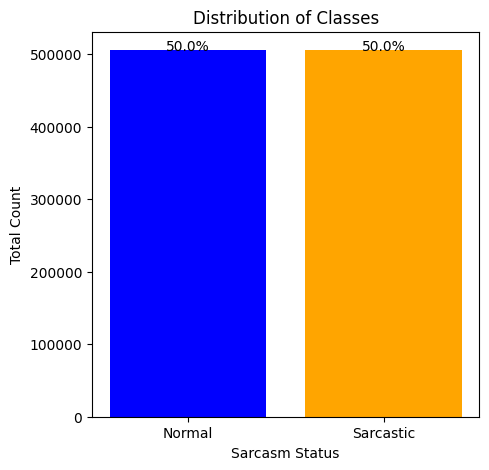
\includegraphics[width=0.5\linewidth]{img/class-dist.png}
    \caption{Class Distribution}
    \label{Fig_1}
\end{figure}

The class distribution plot shows that the dataset is close to perfectly balanced, with both classes appearing in equal proportions. This balanced distribution is a significant advantage 
for model training, as it reduces the risk of bias towards one class over the other. In many real-world classification problems, class imbalance can cause the model to overfit to the 
majority class, making it harder to accurately predict instances of the minority class. However, with an equal split, the model can learn to identify both classes effectively.

From a practical standpoint, this balanced distribution simplifies model evaluation. Metrics such as accuracy, precision, recall, and F1-score will likely give a more reliable indication 
of the model's true performance across both classes. For instance, in an imbalanced scenario, accuracy alone can be misleading if the model simply predicts the majority class most of the 
time. In this case, accuracy is more meaningful, as each class is equally represented. Moreover, the distribution eliminates the need for data augmentation techniques to artificially 
adjust class balance.

For the purpose of this research, I focused on retaining only the labels and comments columns from the dataset, as the other columns did not provide significant contextual value for this 
analysis, as I mentioned earlier.

The next step involved implementing a text preprocessing function to prepare the comments for model evaluation. First, the function converts all letters to lowercase and removes any unnecessary spaces to create a uniform format. 
Afterwards, it addresses contractions using the "contractions" Python library. This process transforms shortened forms of words or combinations of words (e.g., "don't" becomes "do not") 
for better processing.

I also considered lemmatization, which is a process that reduces words to their dictionary form (e.g., "running" becomes "run"). However, I decided against using this technique because 
it negatively impacted model performance. Lemmatization can sometimes eliminate various sarcastic nuances, as certain words can carry different meanings depending on their grammatical form.

Additionally, I removed newline characters to maintain a continuous flow of text. I also inserted spaces to separate words from punctuation marks and replaced any instances of more than 
two consecutive spaces with a single space. This preprocessing function was then applied to the entire comments column.

I also conducted an analysis on comment length distribution, displayed in Figure \ref{Fig_2}, to examine how the lengths of both normal and sarcastic comments are distributed within the 
dataset.

\begin{figure}
    \centering
    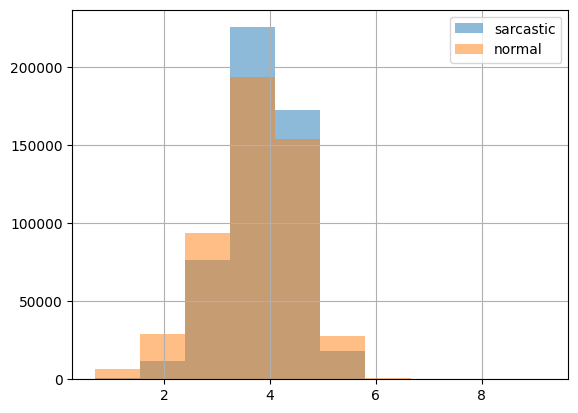
\includegraphics[width=0.5\linewidth]{img/length-dist.png}
    \caption{Comment Length Distribution}
    \label{Fig_2}
\end{figure}

It can be observed that most comments fall within a relatively short length range, with the highest concentration between 3 and 5 words. The peak around this range indicates that both 
normal and sarcastic comments share a similar length distribution, as their overlapping bars show nearly identical trends.

Interestingly, while there are some longer comments in the dataset, their frequency is significantly lower. Beyond a length of 6 words, the number of comments drops off steeply, and 
comments exceeding 8 words appear to be very rare. This suggests that most of the text samples in the dataset are short, reflecting the nature of user-generated comments on social media 
platforms. The near-identical distribution between the two classes also implies that sarcasm in this dataset is not necessarily linked to longer comments, but rather to the choice of 
specific words or acronyms.

The balanced distribution of comment lengths between sarcastic and normal comments ensures that the model will not develop a bias towards identifying sarcasm simply based on comment 
length. This characteristic makes it necessary for the model to rely on deeper linguistic patterns to effectively distinguish between the two classes.

    \section{Methodology}

In this section, I will detail the analysis methods used in my research, including model selection, parameter settings, and validation strategies.

To begin, I conducted a train-test split on the dataset, where I divided the data into training and testing sets with a ratio of 80:20. 
This split was chosen to ensure that there is a substantial amount of data for training the models while retaining a sufficient portion for testing their generalization capabilities. 
An 80:20 split is a common practice in machine learning, providing a good balance between training performance and validation accuracy. By allocating 80\% of the data for training, 
the models can be adequately trained capture the underlying patterns in the data. The remaining 20\% serves as an unbiased test set to evaluate the models performance on unseen data.

\subsection{Machine Learning Methodology}

To evaluate the models performances, I used a 5-fold cross-validation strategy using "StratifiedKFold", ensuring that each fold preserves the percentage of samples for each class. 
This method enhances the reliability of performance estimates by mitigating the variance associated with a single train-test split. Cross-validation provides multiple performance 
estimates, which gives a better understanding of how the models will perform in practice. The choice of 5 folds strikes a balance between bias and variance: while more folds can 
provide better estimates, they also require more computational resources and can lead to longer training times. The metrics evaluated during cross-validation included accuracy, 
F1 score, recall, and precision.

For this part of the research, I experimented with two distinct text representation techniques: Term Frequency-Inverse Document Frequency (TF-IDF) and Bag of Words (BoW). 
For the TF-IDF vectorization, I utilized the TfidfVectorizer, configuring it to extract n-grams ranging from unigrams to trigrams while limiting the maximum number of features to 50,000. 
This configuration was chosen to capture both individual words and phrases that may convey sarcasm, allowing the model to leverage contextual information effectively. 
Similarly, for the BoW representation, I used CountVectorizer with the same n-gram range and feature limit. Both representations enable the models to learn from the frequency of terms, 
helping them identify patterns indicative of sarcasm.

I tested four machine learning models: Logistic Regression and Ridge Classifier, each applied to both TF-IDF and BoW representations. The Logistic Regression model was configured with 
a regularization parameter "C" set to 0.5 and L2 penalty, while the Ridge Classifier was set with an alpha parameter of 1.0. The choice of "C" was based on prior research indicating that 
moderate regularization often yields better performance in text classification tasks by preventing overfitting. The L2 penalty further enhances model generalization by constraining the 
coefficients. For the Ridge Classifier, the alpha parameter of 1.0 was selected to provide a strong regularization effect while still allowing the model to capture significant features 
in the data, ensuring balanced performance.

After evaluating the models, I calculated the mean and standard deviation of the metrics across the folds to provide an assessment of each model's performance. This approach not only 
helps in identifying the best-performing model but also in understanding the stability and reliability of the results. Additionally, I generated confusion matrices to visualize each 
model's classification results, which aids in understanding misclassifications and the distribution of true positives, false positives, true negatives, and false negatives. 
The best model, according to mainly to accuracy or other metrics in case of an equality, will be trained on the full dataset.
    \section{Results}
In this section, I will present the performance of both the machine learning and deep learning models on the sarcasm detection task. The evaluation metrics include accuracy, F1 score, 
recall, and precision. In addition, confusion matrices provide further insight into each model's performance by detailing the distribution of true positives, true negatives, 
false positives, and false negatives.

\subsection{Machine Learning Models Results}

Table \ref{Table_1} summarizes the performance metrics for the four machine learning models that were tested using both TF-IDF and Bag-of-Words (BoW) representations.

\begin{table}
    \caption{Machine Learning Models Results}
    \label{Table_1}
    \begin{tabular}{ccccc}
        \toprule
            \textbf{Model} & \textbf{Accuracy (\%)} & \textbf{F1 Score (\%)} & \textbf{Recall (\%)} & \textbf{Precision (\%)} \\
        \midrule
            Logistic Regression (TF-IDF)  & 71.9 & 70.7 & 67.7 & 73.9 \\
            Ridge Regression (TF-IDF)     & 71.5 & 70.5 & 68.2 & 73.0 \\
            Logistic Regression (BoW)     & 71.9 & 70.4 & 66.9 & 74.3 \\
            Ridge Regression (BoW)        & 71.2 & 69.5 & 65.7 & 73.8 \\
         \bottomrule
    \end{tabular}
\end{table}

Logistic Regression model with TF-IDF achieved an accuracy of 71.9\% and an F1 score of 70.7\%. The confusion matrix reveals 273,531 true positives and 307,988 true negatives, 
with 96,334 false positives and 130,741 false negatives. While the model demonstrates a reasonably strong performance overall, the relatively high number of false negatives suggests that it sometimes 
fails to detect sarcasm, misclassifying sarcastic comments as normal.

Ridge Regression with TF-IDF achieved slightly lower accuracy at 71.5\% and an F1 score of 70.5\%. This model recorded 275,560 true positives and 302,802 true negatives, 
with 101,520 false positives and 128,712 false negatives. Compared to Logistic Regression (TF-IDF), it is marginally more aggressive in predicting sarcasm, as indicated by the higher 
false positive count, although it does slightly better in terms of capturing sarcastic instances (fewer false negatives).

When using a BoW representation, Logistic Regression obtained an accuracy of 71.9\% and an F1 score of 70.4\%. The confusion matrix shows 270,556 true positives and 310,948 true negatives, 
with 93,374 false positives and 133,716 false negatives. This model correctly classifies a higher number of normal comments, as indicated by the increased true negative count and reduced 
false positives. However, this comes at the cost of a higher number of false negatives, meaning that it misses a greater number of sarcastic comments.

Ridge Regression with BoW achieved an accuracy of 71.2\% and an F1 score of 69.5\%. Its confusion matrix reveals 265,506 true positives and 310,275 true negatives, along with 
94,047 false positives and the highest number of false negatives at 138,766. This model struggles most with detecting sarcastic comments, as evidenced by its high false negative count, 
even though it performs well in correctly identifying normal comments.

Overall, TF-IDF-based models provide a better balance between false positives and false negatives compared to their BoW counterparts. Among these, Logistic Regression with TF-IDF offers 
the best trade-off, achieving high accuracy while minimizing misclassifications. This model was trained on the full dataset and obtained an accuracy of 72.23\%. The confusion matrices 
for the models are available in Figure \ref{Fig_4}.

\begin{figure}
    \centering
    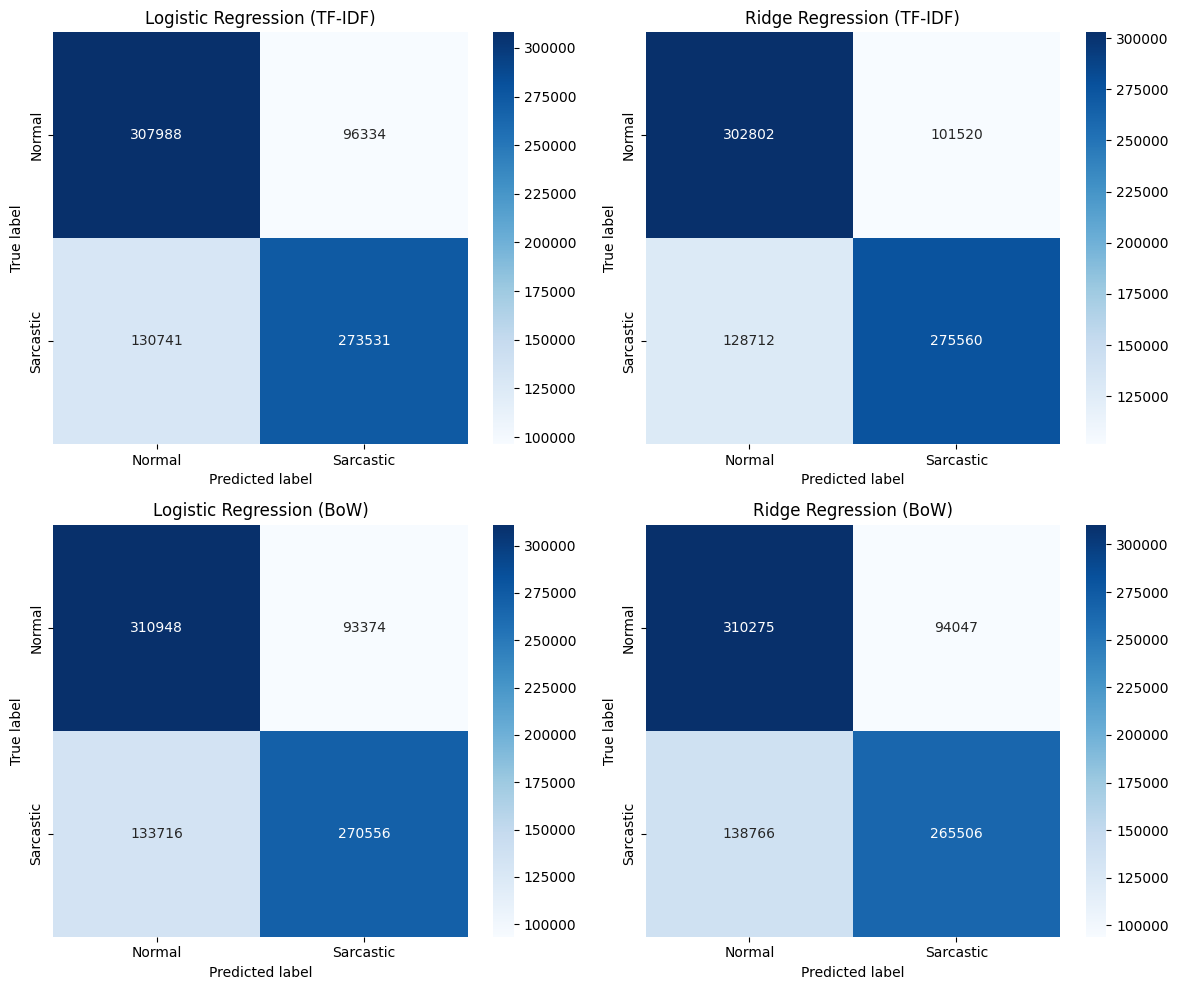
\includegraphics[width=0.8\linewidth]{img/conf_matrix.png}
    \caption{Confusion Matrices}
    \label{Fig_4}
\end{figure}

    \section{Conclusion}

This study aimed to investigate the effectiveness of various machine learning and deep learning models in detecting sarcasm in textual data. 
Specifically, I explored the performance of Logistic Regression and Ridge Regression using both Term Frequency-Inverse Document Frequency (TF-IDF) and Bag-of-Words (BoW) representations, 
alongside Long Short-Term Memory (LSTM) networks utilizing GloVe and Word2Vec embeddings. My findings indicate that TF-IDF-based models, particularly Logistic Regression with TF-IDF, achieved 
the best balance between accuracy and minimizing misclassifications, while BoW-based models tended to struggle more with detecting sarcasm.

On the deep learning front, the LSTM model using Word2Vec embeddings outperformed the one using GloVe, highlighting the importance of word representation in capturing the nuances of sarcasm. 
Overall, while both traditional and deep learning approaches demonstrated reasonable effectiveness in sarcasm detection, the choice of word embeddings and feature representation has shown 
differences in model performance. Future work may focus on refining these models further by incorporating more advanced techniques and additional contextual information to enhance sarcasm 
detection capabilities.

    
    \bibliographystyle{splncs04}
    \bibliography{references}
\end{document}
